\documentclass[letterpaper,12pt]{article}
\usepackage[utf8]{inputenc}
\usepackage{amsmath, amsfonts}
\usepackage[x11names]{xcolor}
\usepackage{pgfplots}
\usepackage{tikz}
\usepackage{braket}

\usetikzlibrary{arrows.meta}
\pgfplotsset{
  compat = newest,
  my_style/.style={
    clip=false,
    axis lines=middle,
    axis equal,
    axis line style={Latex-Latex},
    xmin=-1,
    xmax=1,
    ymin=-1,
    ymax=1,
    xlabel={$x$},
    ylabel={$y$},
    tick style={draw=none},
    ticks=none,
    line width=1pt,
  },
}

% remove spacing around date and author
\usepackage{titling}
\predate{}
\postdate{}
\preauthor{}
\postauthor{}

\author{}
\title{MATH 262 - Homework 7.1}
\date{} % clear date

\begin{document}

\maketitle

\begin{enumerate}
  \item[6.]
    Arguing geometrically, find all eigenvectors and eigenvalues of the linear transformation:
    \begin{center}
      Rotation through an angle of $180^\circ$ in $\mathbb{R}^2$
    \end{center}
    Then find an eigenbasis if you can, and thus determine whether the given transformation is diagonalizable. \\
    \\
    Below is a plot of two vectors in $\mathbb{R}^2$ and their transformed counterparts. \\
    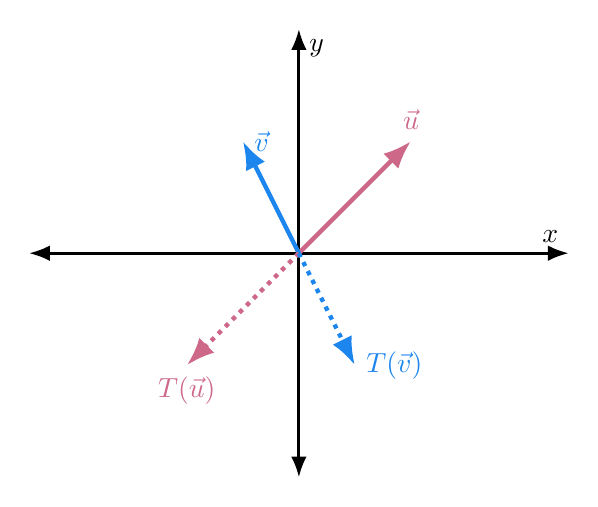
\begin{tikzpicture}
      \begin{axis}[my_style]
        \addplot[-Latex, PaleVioletRed3, ultra thick] coordinates {
          (0, 0)
          (0.5, 0.5)
        } node[above,pos=1] {$\vec{u}$};

        \addplot[-Latex, DodgerBlue2, ultra thick] coordinates {
          (0, 0)
          (-0.25, 0.5)
        } node[right,pos=1] {$\vec{v}$};

        \addplot[-Latex, PaleVioletRed3, ultra thick, dotted] coordinates {
          (0, 0)
          (-0.5, -0.5)
        } node[below,pos=1] {$T(\vec{u})$};

        \addplot[-Latex, DodgerBlue2, ultra thick, dotted] coordinates {
          (0, 0)
          (0.25, -0.5)
        } node[right,pos=1] {$T(\vec{v})$};
      \end{axis}
    \end{tikzpicture} \\
    Notice both $T(\vec{u})$ and $T(\vec{v})$ go in the opposite directions of $\vec{u}$ and $\vec{v}$, respectively, but otherwise remain the same. Therefore, each vector's eigenvalue is $-1$. Thus, the transformation is diagonalizable and the eigenbasis is the basis of $\mathbb{R}^2$ i.e. $\begin{bmatrix}1 \\ 0\end{bmatrix}$, $\begin{bmatrix}0 \\ 1\end{bmatrix}$. All vectors in $\mathbb{R}^2$ are eigenvectors of this transformation.
\end{enumerate}

\end{document}
